\chapter{Literature Review}
An essential part of your project that helps “lift” your project’s academic level is the Review /
Survey of Literature and Related Works; it is the part where you (a) demonstrate your
knowledge of the topic(s) relevant to your project and (b) locate your work in the context of the
rest of the literature. This normally has the form of a chapter in which you introduce and discuss
the theories, concepts and work of others that you use (or have rejected/dismissed) in your
project. 
%Insert figure in the centre of the text at the location you specify (h)
\begin{figure}[h]
\centering
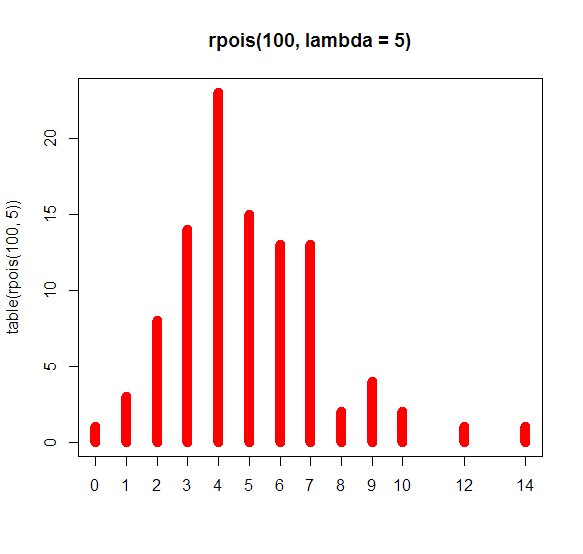
\includegraphics[width=0.5\textwidth]{./images/plotTest01}
\caption{Caption}
\label{fig:plot01}
\end{figure}
The chapter gives you the opportunity to demonstrate how your work fits with the work
others did; it also gives you the opportunity to review and evaluate these in relation to your
project making sure that the extent of your contribution is emphasised. The review should be
directed towards the topics and the themes your project tackles and under no circumstances it
should be a general textbook review.